%%%%%%%%%%%%%%%%%%%% author.tex %%%%%%%%%%%%%%%%%%%%%%%%%%%%%%%%%%%
%
% sample root file for your "contribution" to a contributed volume
%
% Use this file as a template for your own input.
%
%%%%%%%%%%%%%%%% Springer %%%%%%%%%%%%%%%%%%%%%%%%%%%%%%%%%%


% RECOMMENDED %%%%%%%%%%%%%%%%%%%%%%%%%%%%%%%%%%%%%%%%%%%%%%%%%%%
\documentclass[graybox]{svmult}

% choose options for [] as required from the list
% in the Reference Guide

\usepackage{bibentry}
\usepackage{type1cm}        % activate if the above 3 fonts are
                            % not available on your system
%
\usepackage{makeidx}         % allows index generation
\usepackage{graphicx}        % standard LaTeX graphics tool
                             % when including figure files
\usepackage{multicol}        % used for the two-column index
\usepackage[bottom]{footmisc}% places footnotes at page bottom

\usepackage{newtxtext}       % 
\usepackage{newtxmath}       % selects Times Roman as basic font
\usepackage{dirtytalk} \newcommand{\mysay}[1]{\say{\textit{#1}}}
\usepackage{enumerate}
\usepackage[unicode,colorlinks=true,breaklinks,allcolors=black]{hyperref}
\usepackage{cleveref}
\usepackage{ltablex}
\usepackage{booktabs}
\usepackage{hyphenat}
\usepackage{makecell}
\usepackage{doi}
\usepackage{enumitem}


\usepackage{listings}      % Pozwala na używanie kodu w papierze // Marcel Jerzyk



\graphicspath{{img/}}

% Probably should be swapped for JPEGs!
\usepackage{pgfplots}
\pgfplotsset{compat=1.17}
\usepgfplotslibrary{statistics}
\usetikzlibrary{pgfplots.statistics} % LATEX and plain TEX
\usetikzlibrary[pgfplots.statistics] % ConTEXt

%\nobibliography
\usepackage{fixme}

\nobibliography*


% see the list of further useful packages
% in the Reference Guide

\makeindex             % used for the subject index
                       % please use the style svind.ist with
                       % your makeindex program

%%%%%%%%%%%%%%%%%%%%%%%%%%%%%%%%%%%%%%%%%%%%%%%%%%%%%%%%%%%%%%%%%%%%%%%%%%%%%%%%%%%%%%%%%

\usepackage{fancyhdr}

\pagestyle{fancy}
\fancypagestyle{firstpage}{%
  \fancyhf{}% clear default for head and foot
  \lhead{\footnotesize Preprint of a chapter: Marcel Jerzyk, Eryk Krupa, Jakub Litkowski, Jakub Szańca and Lech Madeyski, Developments in Information and Knowledge Management for Business Applications, Studies in Systems, Decision and Control, chapter ”Title” Springer}
}
\setlength{\headheight}{110pt} 

\begin{document}

\title*{Evaluating the potential of a candidate for a job offer based on his GitHub profile}% - deadline 10.10, min. 25 stron do vol. 2 \url{https://www.springer.com/gp/book/9783030621506}}
% Use \titlerunning{Short Title} for an abbreviated version of
% your contribution title if the original one is too long
\titlerunning{Evaluating the potential of a candidate for a job offer based on his GitHub profile.}
\author{Marcel Jerzyk, Jakub Litkowski, Jakub Szańca and Lech Madeyski}
% Use \authorrunning{Short Title} for an abbreviated version of
% your contribution title if the original one is too long
\institute{Marcel Jerzyk, Jakub Litkowski, Jakub Szańca \at Wroclaw University of Science and Technology, Poland
\and Lech Madeyski \at Wroclaw University of Science and Technology, Poland, \email{lech.madeyski@pwr.edu.pl}}
%
% Use the package "url.sty" to avoid
% problems with special characters
% used in your e-mail or web address
%
\maketitle

\thispagestyle{firstpage}

\abstract*{
\noindent\textit{Context:} 
Nowadays it is much harder for new programmers to acquire industry experience. Modern software development demands high levels of technical specialization. These conditions make IT
companies focus on creating cross-functional teams, such as frontend, backend, and mobile developers. In this
context, the success of software projects is highly influenced by the expertise of these teams in each field
\noindent\textit{Objective:} 
This study aims to identify and investigate the current state of the art with respect to: (1) predictors used in prediction models to detect code smells, (2) ... and (6) improvement ideas with regard to code smell detection using ML/AI. 
\noindent\textit{Method:} We conducted a systematic review using a database search in Scopus and evaluated it using the quasi-gold standard procedure to identify relevant studies.
In the data sheet used to obtain data from publications we factor research questions into finer-grained ones, which are then answered on a per-publication basis. Those are then merged over a set of publications using an automated script to obtain answers to the posed research questions. 
\noindent\textit{Results:}
We have identified 45 primary studies relevant to the primary objectives of this research. 
The results show...
\noindent\textit{Conclusion:} 
Only a few smells---Blob, Feature Envy, Long Method and Data Class---...
}

\abstract{
\newline
\noindent\textit{Context:} Nowadays it is much harder for new programmers to acquire industry experience. This trend started being noticeable at around 2018 \cite{FluffJobsRojewska18} but now - due to coronavirus pandemic - it is even more prominent \cite{MoneyLukasik2020}. Several dozen of junior programmers apply for one job offer \cite{KodillaZoellner2020} and thus there can be a need for a tool that would facilitate the identification of candidates that the employer is interested in. It is considered a good practice for Junior Developers that are seeking to be hired to have public repositories with some of their personal work. The problem is that usually recruiters does not have the knowledge to make use of that information which in fact could be very impactfull as it is literally the "show-off" of one's current skills. Right now it is completely disregarded until the later stages of recruitment phase - after the junior already passes the first recruiter look-up. Only then the repository is examined by a technical interviewer but that also could be a concern for the company as it books-out the valuable time of an expertised employee. Also there could be situations when one's CV is completely skipped due to various reasons and thus missing the chance to be employed or have his repositories examined by a professional which could prove otherwise (that one has all the  abilities and skills needed for the position).
\newline
\noindent\textit{Objective:} 
This study aims to identify and investigate if its possible to acquire use-full information's from a GitHub profile that could be beneficial for recruiters in a recruitment process. If that would be proven to be effective way of measuring one's abilities and skills - maybe it could be also used by the developers themselves to atest their own potential quality. 
\newline
The visible main challenge is inefficient hiring process with no accurate technical screening methodology. Overall goal is to improve the rate of recruiting highly skilled programmers by making use of the in formations that are already provided in CV's by standard.
\newline
\noindent\textit{Method:} We conducted a systematic review using a database search in Scopus and evaluated it using the quasi-gold standard procedure to identify relevant studies. 
We created polls to gather information from developers own experiences and asked them to attach their GitHub profiles to the questionnaire. Then, with machine-learning based approach, we used that data to automatically evaluate the potential of a candidate by giving only the link to GitHub profile on input.
In the data sheet used to obtain data from publications we factor research questions into finer-grained ones, which are then answered on a per-publication basis. Those are then merged over a set of publications using an automated script to obtain answers to the posed research questions. 
\newline
\noindent\textit{Results:}
...
\newline
\noindent\textit{Conclusion:} 
...
}

%\keywords{code smells \and antipatterns \and machine learning \and predictive modelling \and systematic review}


%\section{Introduction}

While hiring practices of graduates are not thoroughly studied in the context of
the IT industry, the concept in general is well understood
Selecting the most valuable candidate for interview is an important process. While hiring practices of graduates are not thoroughly studied in the context of the IT industry, the concept in general is well understood \cite{HiringProcess}. As a standard, recruiters look through Curriculum Vitae (\emph{CV}) to categorize all candidates and call them for interview. Nowadays, to minimize the time spent on a single CV, recruiters have various pre-screening methods, listing them in order of importance \cite{SantanderCVLectureScholarship}:
\begin{itemize}
  \item employment history and previously business-related work
  \item university and academic performance
  \item listed programming abilities and other colloquially called \emph{"buzzwords"}
  \item soft skills
\end{itemize}

The CV could include a lot of important information's but the recruiter usually spends from 6 to 60 seconds at max per one application \cite{SantanderCVLectureScholarship}. It is surely not enough time to examine candidate skills correctly, more over - the recruiters usually doesn't even have the industrial knowledge to asses the skills and examine candidate's quality by browsing through "code portfolio". It is done only after the pre-screening is already done, when the filtered-out list of candidates goes to a professional technical employee that has the required knowledge and skills to examine the potential of a candidate. The information is there - various online hosting websites that allow to showcase one's code are widely used and added to the CV's - but a qualified candidate may be omitted in the pre-screening method because his cv-building skills were not good enough to pass.

One of such hosting websites is GitHub \footnote{GitHub Website URL: https://github.com/} - it is a service supporting version control using git, which is used by programmers and developers for storing and managing theirs code-base repositories. The popularity of GitHub in 2021 is well established and still rising. Already in 2020 the website gathered over 36 million users \cite{GitHubUsers2020} and today, as of March 2021 - there are 55 million users \cite{GitHubUsers2021}. Dabbish et al. \cite{DabbishC} showed that software developers in public project on GitHub consciously manage their online reputation. They do recognise that others developers can assess their personal characteristics such as the quality of work or commitment by looking for example through their commits and judging the quality, checking the amount of forks of an project or stars. Singer et al. \cite{Singer} found that the amount of followers one have on GitHub is also an valuable information.

We recognise that the CV evaluation procedure has several shortcomings and not much has changed since 2013 \cite{Capiluppi}. These shortcomings especially apply for those who do not have any relevant work experience or formal degree. We also note that GitHub is a place storing lots of very valuable informations that could (or maybe should) be used to evaluate potential of a candidate. Various research works have confirmed that it is possible to retrieve data like technical technical role \cite{TechnicalRole}, identifying Experts in Software Libraries and Frameworks \cite{SoftwareLibraries} .Because the recruiters have very limited time available to review a single CV, we search for an machine-learning based solution that could help extract the information from GitHub by a non-expertised recruiter. This could not only reduce the amount of false-positive skips but also increase the overall quality of list of candidates after the pre-screening is done.

\section{Introduction}

While hiring practices of graduates are not thoroughly studied in the context of
the IT industry, the concept in general is well understood
Selecting the most valuable candidate for interview is an important process. While hiring practices of graduates are not thoroughly studied in the context of the IT industry, the concept in general is well understood \cite{HiringProcess}. As a standard, recruiters look through Curriculum Vitae (\emph{CV}) to categorize all candidates and call them for interview. Nowadays, to minimize the time spent on a single CV, recruiters have various pre-screening methods, listing them in order of importance \cite{SantanderCVLectureScholarship}:
\begin{itemize}
  \item employment history and previously business-related work
  \item university and academic performance
  \item listed programming abilities and other colloquially called \emph{"buzzwords"}
  \item soft skills
\end{itemize}

The CV could include a lot of important information's but the recruiter usually spends from 6 to 60 seconds at max per one application \cite{SantanderCVLectureScholarship}. It is surely not enough time to examine candidate skills correctly, more over - the recruiters usually doesn't even have the industrial knowledge to asses the skills and examine candidate's quality by browsing through "code portfolio". It is done only after the pre-screening is already done, when the filtered-out list of candidates goes to a professional technical employee that has the required knowledge and skills to examine the potential of a candidate. The information is there - various online hosting websites that allow to showcase one's code are widely used and added to the CV's - but a qualified candidate may be omitted in the pre-screening method because his cv-building skills were not good enough to pass. 

One of such hosting websites is GitHub \footnote{GitHub Website URL: https://github.com/} - it is a service supporting version control using git, which is used by programmers and developers for storing and managing theirs code-base repositories. The popularity of GitHub in 2021 is well established and still rising. Already in 2020 the website gathered over 36 million users \cite{GitHubUsers2020} and today, as of March 2021 - there are 55 million users \cite{GitHubUsers2021}. Dabbish et al. \cite{DabbishC} showed that software developers in public project on GitHub consciously manage their online reputation. They do recognise that others developers can assess their personal characteristics such as the quality of work or commitment by looking for example through their commits and judging the quality, checking the amount of forks of an project or stars. Singer et al. \cite{Singer} found that the amount of followers one have on GitHub is also an valuable information.

We recognise that the CV evaluation procedure has several shortcomings and not much has changed since 2013 \cite{Capiluppi}. These shortcomings especially apply for those who do not have any relevant work experience or formal degree. We also note that GitHub is a place storing lots of very valuable informations that could (or maybe should) be used to evaluate potential of a candidate. Various research works have confirmed that it is possible to retrieve data like technical technical role \cite{TechnicalRole}, identifying Experts in Software Libraries and Frameworks \cite{SoftwareLibraries} .Because the recruiters have very limited time available to review a single CV, we search for an machine-learning based solution that could help extract the information from GitHub by a non-expertised recruiter. This could not only reduce the amount of false-positive skips but also increase the overall quality of list of candidates after the pre-screening is done. 

\section{Systematic Review}

What distinguishes this paper among others — as we mentioned — we do recognize that the majority of recruiters does not have skills that could examine the technicality of a candidate. For example in the \emph{"Mining the Technical Roles of GitHub Users"} the survey was conducted among recruiters from StackOverflow website \footnote{StackOverflow Website URL: https://stackoverflow.com/} - which is primarily used by developers for the purposes of collaboration \& knowledge sharing. Thus, it can be concluded that the surveyed sample was exceptional among global population of recruiters as they have made extra efforts to create an account on IT-technical website and not only that - they were actively browsing it and even possibly creating extra content which made them visible and reachable by researchers. Based on the research we have conducted, there are only a few unfinished recommendation systems that use the user GitHub profile but at the same time there is some research that focuses on mining the data from the repositories.

\subsection{Research Questions}
Research questions presented below should explain to help understand the importance of creating such tool and also provide an information about the functionalities which potential end user might need (i.e. - recruiters, developers themselves). Furthermore we also explore issues related to the recruitment itself, as well as the quality of repositories.

Hence, we defined four research questions.
\begin{itemize}
\item{\emph{RQ1: What are the most common skills the company is looking for among the candidates?}\\
  Our system needs to determine whether developer is worthy of attention and if he should be considered further in the recruitment process. The answer to this question should explain what skills are considered important among companies. }
\item{\emph{RQ2: How a given repository makes a good impression?}\\
  One way of assessing developer expertise is to analyse his projects. Thus, we should determine which features of repositories are the most representative ones.} 
\item{\emph{RQ3: Is it possible to get a good enough information about the candidate's potential based on the GitHub profile?}\\
  This question should provide us with information whether the recommendation system based on repositories is worth devoting time.} 
\item{\emph{RQ4: Is Github repository used only for programming purposes?}\\
  It often happens that an item is used contrary to the original intention of the author. Same situation might occur with the repositories. There is no compulsion to prohibit the use of a repository for purposes other than development.}
\end{itemize}

\subsection{Currently Available Resources on the Subject}
We used search engines (Google Scholar and Scopus) in order to find proper resources and currently available papers on the subject that is investigated by our paper. We searched the studies we received using pre-defined search string which is given below~\ref{lst:search-string}.

\begin{lstlisting}[language=Python, label={lst:search-string}]
( 
  skill AND
  repository AND
  ( github  OR  gitlab  OR  bitbucket )
) OR (
  recruitment  OR hiring  OR interview
) AND (
  programming AND purpose 
) AND ( 
  "Computer science"
) AND ( 
  mining AND software
)
\end{lstlisting}
Because of enormous number of results in Scopus we decided to add another limitations such as exact keyword: "Software Engineering" and years of publication: 2017-2021.


This gave us a good amount of publications which needed to be further filtered by hand. Unfortunately, many of them did not answer the previously established research questions and also many of them were not in English language. As shown on the~\ref{fig:literature-identification} search engines provided us with over two hundred publications. In the end, we've identified ten of the most important studies that are helpful in our topic.

\begin{figure}[htp]
\centering
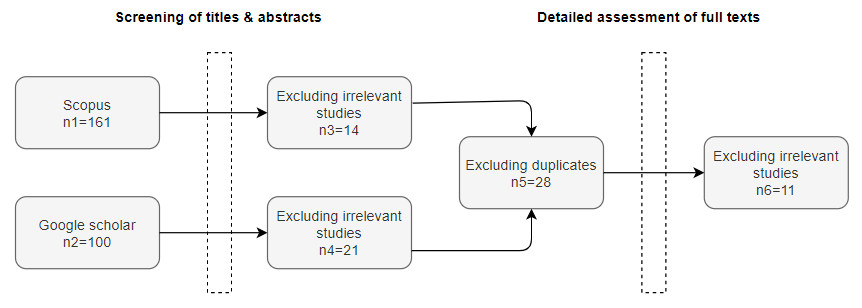
\includegraphics[width=11cm]{searchProcess11.2}
\caption{Literature identification}
\label{fig:literature-identification}
\end{figure}

\subsection{Results Selection Process}
After running the search string query, we were presented with a large number of results. We have went through the results list and discarded all duplicate entries and simultaneously discarded those papers whose titles or abstracts were not related to the topic of our research. Thus, we ended up with 28 papers which we further examined. Finally, we have chosen 10 papers which are closely related to the subject of this paper.


\section{Literature Review}
Choosed literature gives us answears to the questions asked earlier in this paper and provide us some useful informations. \\Skills which are needed from IT specialists descirbes \cite{StackOverflowStudies} based on job offers posted on Stack Overflow. They extract needed data and then define which hard and soft skills are welcome among recruiters. This study helps us to depict usefull skills and also can help young programmers to find their first dream job as a software engineer. Paper \cite{DoOnBoardingProgramsWork} gives us a very interesting look on boarding programs. It aware us that not every contribiutor to the open source systems is going to be a skilled programer. Based on this article many contributors are people who took part in a boarding program which are mentored by some master. Master gives participants many tips and helps them with their problems. Having that information we should be careful looking at repository contributors because not everyone is going to be professional. Article \cite{GitHubProfilesToJobAdv} shows us how skills extracted from job offers can be matched with developers skills extracted from repositories. Description of data scraping and how matching can be done should be useful in system which is presented in this paper.
\\Subject of repositories is discussed in \cite{MiningGitHub}, they take a deep look into the structure and usage of repositiories. This paper points out that not every repository is used for programming porpuses. Many of the repositories are abandonded few weeks after creation which causes very large actvity in first weeks but with the time passing, activity is decreasing drastically. A good amount of peple are using repositories as a storage or they simply have empty repositories as an effect of some experiments or attempts of learning. 
\\Recruitment process is described by the developers in paper \cite{HiringIsBroken} where authors collected data from actuall developers who posted their opinions on social networks. There is said that recruiment process casues a lot of stress and is not liked among developers. Programmers say that during the interview they can not show their whole potential and they are served with excercises which are not useful during normal work and do not check their actuall knowleadge. Developers criticise big companies for their ease of rejecting canditates beacause there are going to be much more candidates and it is not going to be a big mistake if they reject someone good - simply they will find someone else.
\\In recent years there have been carried out a various similar types of research concerning issues related to our study. For instance, there was created an online developer profiling tool assessing developer expertise \cite{GitLabProfilingTool}. The tool considers factors such as code quality, code quantity, contribution to rank  software engineer’s repositories and his skills as well. Evaluations of developers using greater number of features were determined as more accurate ones. However, weight of all of the indicators was equivalent, so none of them could be chosen as the most significant. Moreover, the tool is based on analysis of repositories created on GitLab which is definitely less popular than GitHub \cite{GitLabvsGithub}.
\\Furthermore, a relation between technical and social skills \cite{WhatMakesGoodDev} was explored also. In the study which aims at finding out what makes developer good we discovered that there is a lack of strong association between above types of skills, so doubtless it is extremely tough to assess soft and social skills mining GitHub repositories.
\\Generally, candidate selection process might be based on LinkedIn profile, CV and Github Profile as well \cite{CandidateSelection}. Although it could be complicated to obtain information about non-technical skills using above resources, personality traits of candidates could be accessed from analyzed transcription of a phone call.
\\In terms of identifying experts in software libraries and frameworks \cite{SoftwareLibraries} it was analyzed which features best distinguish library specialists. First of all, it was explored that the feature values are different for experts in each library. Nevertheless, the features such as number of commits are always relevant.


\section{Methodology}
In this section we defined methods, techniques, tools and processes referring to the main part of our research.
\subsection{Data Collection}

\subsubsection{Questionnaire}

Our main goal during the data collection process was to obtain GitHub Usernames along with as many answers to questions related to the subject of the recruitment process, assessment of own skills as well as some additional information which could help in the reconstruction of results found in other papers. We have created a Google Form questionnaire and then posted it on two programming-related Facebook Groups.

In both groups, one can find people with a full range of professional experience but based on the activity (posts and comments), one of them is mainly characterized by highly qualified employees (Seniors) while the other seems evenly distributed.

\subsubsection{Parsing GitHub Information}

To collect data from GitHub we used GraphQL Queries \footnote{GraphQL GitHub API: https://docs.github.com/en/graphql}. The query takes only the username on input and on output puts only the information precisely specified within the query itself. GraphQL Query is presented in~\ref{lst:graphql-query} and output format in~\ref{lst:graphql-output-json}.


\begin{lstlisting}[language=R, label={lst:graphql-query}]
{ repositoryOwner(login:"<USER_NAME>") {
    repositories(first: 5, orderBy: {
        field:PUSHED_AT,direction:DESC},
        isFork:false) {
      edges { node {
          name
          diskUsage
          forkCount
          isEmpty
          languages(first : 10){
            edges { size node {
                name
              }
            }
          }
          labels(first : 50){
            totalCount
            nodes{
              name
              description
              updatedAt
            }
          }
          issues (first : 20){
            totalCount
            edges { node {
                body
                author {
                  login
                }
              }
            }
          }
          stargazers {
            totalCount
          }
          description
          defaultBranchRef {
            target{ ... on Commit {
                history(first : 10){
                  totalCount
                  edges { node {
                      ... on Commit {
                        message
                        committedDate
                        author{
                          user{
                            login
    } } } } } } } } } } } }
    ... on User {
      bio
      company
      isHireable
      isViewer
    }
  }
}
\end{lstlisting}

\begin{lstlisting}[language=Python, label={lst:graphql-output-json}]
FUTUREOUTPUT
\end{lstlisting} 

\begin{figure}[htp]
\centering
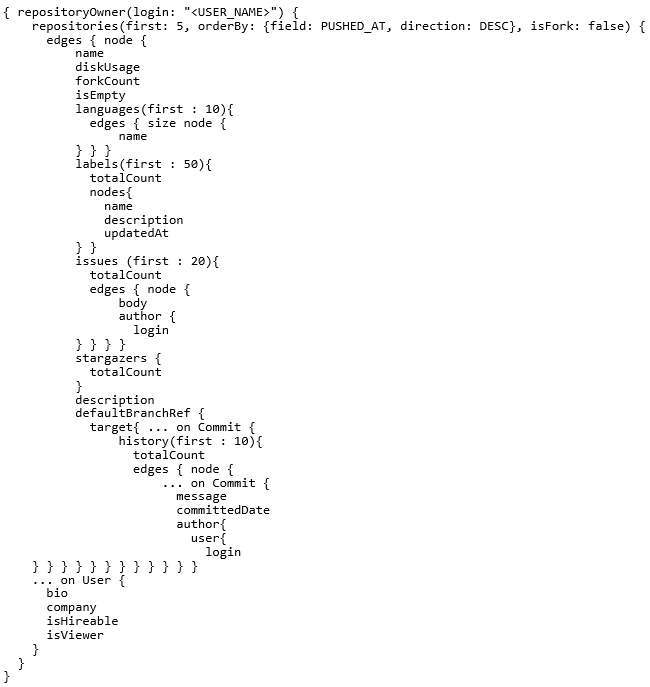
\includegraphics[width=11cm]{query}
\caption{GraphQl Query}
\label{fig:GraphQlQuery}
\end{figure}

\subsection{Data Preprocessing}

\subsubsection{Questionnaire}

In total, we received 67 completed questionnaires and 45 of them were provided with GitHub profile. The data file was further cleaned and reformatted with the use of Python \footnote{Python Website: https://www.python.org/} script. Both the original and formatted CSV files can be found in the project source under the name \emph{,,questionnaire.csv''} and \emph{,,cleaned\_data.csv''} as well as the Python script used for data formatting can be found in \emph{,,py\_scripts''} directory under the name ,,questionnaire\_adjuster.py''. To run the script, one must have Python 3.9 or newer installed on the machine along with "Numpy" \footnote{Numpy PyPI Page - https://pypi.org/project/numpy/}, "Pandas" \footnote{Pandas PyPI Page - https://pypi.org/project/pandas/} and "Requests" \footnote{Requests PyPI Page - https://pypi.org/project/requests/} packages.

\subsubsection{Repositories}

One of the most difficult tasks is to properly obtain information from the repositories of a given user. For research purposes, we decided to track them for potential errors and warnings which can be identified via linters. Linter is a static code analysis tool used to flag any bugs, errors, stylistic warnings, suspicious constructs, redundant code and more depending on the language and/or tool. Of course, the user could have repositories with code written in any language that exists, and that is a real problem, which we mitigated by a linter-aggregating tool - \emph{Mega Linter} \footnote{MegaLinter GitHub Page - https://github.com/nvuillam/mega-linter}. Mega Linter is an open-source tool that simply detects the languages used in a given project and then uses all available linters to scan it through. After the scan, it prints out a summary table with the number of Files that were detected and scanned with a given linter, the number of fixed files automatically during the run time, and the number of errors that couldn't be automatically fixed. There's also a second table that's printed somewhere in the first half of the output log that has information about detected duplicate lines and tokens in the project. To obtain that data we redirected the output stream into a file and then parsed it with Python script \emph{,,scrape.py''} which can be found in \emph{,,py\_scripts''} folder.

The usage of the Mega Linter and scrape script is more widely described in the main \emph{README.md} file although, in short, one must have Docker \footnote{Docker Website - https://www.docker.com/} and Python installed. Then, simply navigate to the repository which you would like to lint and run a command \ref{lst:shell-command-run-linter} which will generate an \emph{output.txt} file.

\begin{lstlisting}[language=Bash, label={lst:shell-command-run-linter}]
npx mega-linter-runner --flavor all
                  -e 'ENABLE=,DOCKERFILE,MARKDOWN,YAML'
                  -e 'SHOW_ELAPSED_TIME=true'
                 > output.txt
\end{lstlisting}

Copy the file and paste it in the \emph{scrape.py} directory. Finally use \ref{lst:shell-command-scrape-py} command which will generate an \emph{output.json} with a list of dictionaries structured as in \ref{lst:scrape-py-output-example}.

\begin{lstlisting}[language=Bash, label={lst:shell-command-scrape-py}]
python scrape.py -f output.txt
\end{lstlisting}

\begin{lstlisting}[language=Python, label={lst:scrape-py-output-example}]
{
 "language": str,
 "linter": str,
 "files": int or str, #detected files in given language 
 "fixed": int,        #fixed errors automatically
 "errors": int        #errors that could not be fixed
},

or

{
 "language": str,
 "files": int,        #in a given language
 "lines": int,        #in a given language
 "tokens": int,       #("chars") in a given language
 "clones": int,
 "duplicate_lines_num": int,
 "duplicate_lines_percent": float,
 "duplicate_tokens_num": int,
 "duplicate_tokens_percent": float
},
\end{lstlisting}

\subsection{Creating a Machine Learning Model}
Essentially, we decided to chose mlr \footnote{mlr Website: https://mlr.mlr-org.com/} package as a tool which is supposed to help us in creating a machine learning model and which is one of the best machine learning packages in R. \footnote{R Website: https://www.r-project.org/}We determined that we wanted to perform a binary classification, hence we performed the following processes

Firstly, we imported data from csv file with appropriate encoding. We saved selected columns from imported data into a data frame as well. Then, as a first approach we split the data into two datasets in a given ratio: training set - 75\% of data, test set – 25\% of data. Finally, the datasets were prepared and ready to use. The first step toward creating a machine learning model was to define a learning task for a classification. We specified task ID, data used in process and a target column, which had to be a factor, with a \emph{makeClassifTask()} method. Subsequently, we constructed a learner by calling \emph{makeLearner()} method. We needed to choose a classification algorithm. In the beginning, \emph{randomForest} was selected. Afterwards, we trained the model with a \emph{train()} method. We were supposed to specify train subset, use defined task and learner. In the end, we predicted the target values for test dataset. We had to specify using machine learning model and task with a \emph{predict()} method as well. Moreover, by calling \emph{makeResampleDesc()} method we used a cross-validation in order to estimate precisely how accurately a predictive model will perform in practice.


%\input{sections/methods.tex}

%\subsection{Results}
\label{sec:results}

We decided to compare the results for three different models. Below you can find two tables - one of them is based on the results which were achieved using all the available data sources we have (which includes the questionnaire) \textit{[ref: table\ref{table:1}]}  while the other uses only the data that can be gathered using GraphQL request to GitHub API and the Mega Linter with parsing scripts \textit{[ref: table\ref{table:2}]}. In the second case, we used \code{AvgCommitTime}, \code{DupLinesPercent} and \code{LinesPerFile} attributes. Below the tables, we present the correlation matrix of individual features \textit{[ref: figure\ref{fig:correlation-matrix}]}. 

\begin{table}[h!]
\centering
\begin{tabular}{ | m{5em} | m{5em}| m{5em} | m{5em}| m{5em} | m{5em}| } 
\hline
 Algorithm & \textbf{MMCE} & \textbf{MCC} & \textbf{F1} & \textbf{ACC} & \textbf{Kappa}\\ 
 \hline
 \textbf{Random Forest} & 0.329 & 0.245 & 0.410 & 0.671 & 0.219 \\ 
\hline
 \textbf{SVM} & 0.315 & 0.356 & 0.422 & 0.685 & 0.311 \\ 
\hline
 \textbf{KNN} & 0.388 & 0.224 & 0.431 & 0.611 & 0.184\\ 
\hline
\end{tabular}
\caption{Measures scores for each classifiers (all features)}
\label{table:1}
\end{table}

\begin{table}[h!]
\centering
\begin{tabular}{ | m{5em} | m{5em}| m{5em} | m{5em}| m{5em} | m{5em}| } 
\hline
 Algorithm & \textbf{MMCE} & \textbf{MCC} & \textbf{F1} & \textbf{ACC} & \textbf{Kappa}\\ 
 \hline
 \textbf{Random Forest} & 0.360 & 0.299 & 0.451 & 0.639 & 0.245 \\ 
\hline
 \textbf{SVM} & 0.319 & 0.314 & 0.451 & 0.680 & 0.280 \\ 
\hline
 \textbf{KNN} & 0.367 & 0.237 & 0.484 & 0.632 & 0.209\\ 
\hline
\end{tabular}
\caption{Measures scores for each classifiers (\emph{GitHub API} and \emph{Mega Linter} features)}
\label{table:2}
\end{table}

\begin{figure}[htp]
\centering
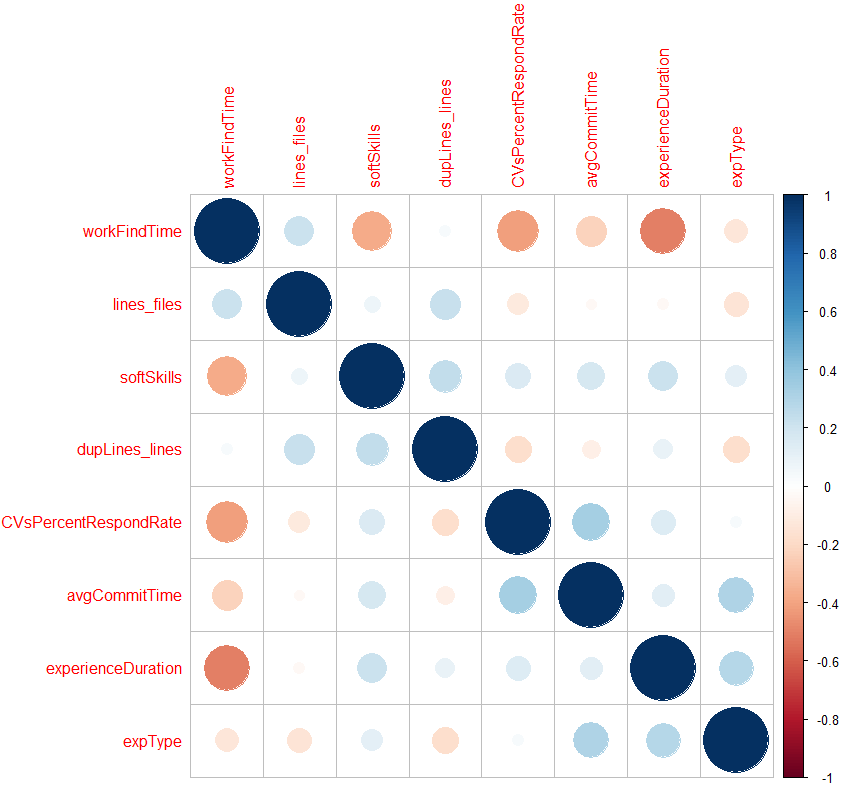
\includegraphics[width=\linewidth]{r_plot_corrrelation.png}
\caption{Correlation Matrix}
\label{fig:correlation-matrix}
\end{figure}


%\subsection{Discussion}
\label{sec:discussion}

The variables prepared for the machine learning model were not correlated with each other. No substantial correlation was observed between the percentage of duplicate lines and the time until the first job was found. Unnoteworthy although reassuring connection, which has the highest correlation among those all variables, between the experience duration and \code{WorkFindTime} is present. 


%\subsection{Conclusions}
\label{sec:conclusions}

\begin{acknowledgement}
\item {This research was ...}
\end{acknowledgement}

\bibliographystyle{plain}
\bibliography{refs}

%%%%%%%%%%%%%%%%%%%%%%%%% referenc.tex %%%%%%%%%%%%%%%%%%%%%%%%%%%%%%
% sample references
% %
% Use this file as a template for your own input.
%
%%%%%%%%%%%%%%%%%%%%%%%% Springer-Verlag %%%%%%%%%%%%%%%%%%%%%%%%%%
%
% BibTeX users please use
% \bibliographystyle{}
% \bibliography{}
%
\biblstarthook{References may be \textit{cited} in the text either by number (preferred) or by author/year.\footnote{Make sure that all references from the list are cited in the text. Those not cited should be moved to a separate \textit{Further Reading} section or chapter.} If the citatiion in the text is numbered, the reference list should be arranged in ascending order. If the citation in the text is author/year, the reference list should be \textit{sorted} alphabetically and if there are several works by the same author, the following order should be used:
\begin{enumerate}
\item all works by the author alone, ordered chronologically by year of publication
\item all works by the author with a coauthor, ordered alphabetically by coauthor
\item all works by the author with several coauthors, ordered chronologically by year of publication.
\end{enumerate}
The \textit{styling} of references\footnote{Always use the standard abbreviation of a journal's name according to the ISSN \textit{List of Title Word Abbreviations}, see \url{http://www.issn.org/en/node/344}} depends on the subject of your book:
\begin{itemize}
\item The \textit{two} recommended styles for references in books on \textit{mathematical, physical, statistical and computer sciences} are depicted in ~\cite{science-contrib, science-online, science-mono, science-journal, science-DOI} and ~\cite{phys-online, phys-mono, phys-journal, phys-DOI, phys-contrib}.
\item Examples of the most commonly used reference style in books on \textit{Psychology, Social Sciences} are~\cite{psysoc-mono, psysoc-online,psysoc-journal, psysoc-contrib, psysoc-DOI}.
\item Examples for references in books on \textit{Humanities, Linguistics, Philosophy} are~\cite{humlinphil-journal, humlinphil-contrib, humlinphil-mono, humlinphil-online, humlinphil-DOI}.
\item Examples of the basic Springer Nature style used in publications on a wide range of subjects such as \textit{Computer Science, Economics, Engineering, Geosciences, Life Sciences, Medicine, Biomedicine} are ~\cite{basic-contrib, basic-online, basic-journal, basic-DOI, basic-mono}. 
\end{itemize}
}

\begin{thebibliography}{99.}%
% and use \bibitem to create references.
%
% Use the following syntax and markup for your references if 
% the subject of your book is from the field 
% "Mathematics, Physics, Statistics, Computer Science"
%
% Contribution 
\bibitem{science-contrib} Broy, M.: Software engineering --- from auxiliary to key technologies. In: Broy, M., Dener, E. (eds.) Software Pioneers, pp. 10-13. Springer, Heidelberg (2002)
%
% Online Document
\bibitem{science-online} Dod, J.: Effective substances. In: The Dictionary of Substances and Their Effects. Royal Society of Chemistry (1999) Available via DIALOG. \\
\url{http://www.rsc.org/dose/title of subordinate document. Cited 15 Jan 1999}
%
% Monograph
\bibitem{science-mono} Geddes, K.O., Czapor, S.R., Labahn, G.: Algorithms for Computer Algebra. Kluwer, Boston (1992) 
%
% Journal article
\bibitem{science-journal} Hamburger, C.: Quasimonotonicity, regularity and duality for nonlinear systems of partial differential equations. Ann. Mat. Pura. Appl. \textbf{169}, 321--354 (1995)
%
% Journal article by DOI
\bibitem{science-DOI} Slifka, M.K., Whitton, J.L.: Clinical implications of dysregulated cytokine production. J. Mol. Med. (2000) doi: 10.1007/s001090000086 
%
\bigskip

% Use the following (APS) syntax and markup for your references if 
% the subject of your book is from the field 
% "Mathematics, Physics, Statistics, Computer Science"
%
% Online Document
\bibitem{phys-online} J. Dod, in \textit{The Dictionary of Substances and Their Effects}, Royal Society of Chemistry. (Available via DIALOG, 1999), 
\url{http://www.rsc.org/dose/title of subordinate document. Cited 15 Jan 1999}
%
% Monograph
\bibitem{phys-mono} H. Ibach, H. L\"uth, \textit{Solid-State Physics}, 2nd edn. (Springer, New York, 1996), pp. 45-56 
%
% Journal article
\bibitem{phys-journal} S. Preuss, A. Demchuk Jr., M. Stuke, Appl. Phys. A \textbf{61}
%
% Journal article by DOI
\bibitem{phys-DOI} M.K. Slifka, J.L. Whitton, J. Mol. Med., doi: 10.1007/s001090000086
%
% Contribution 
\bibitem{phys-contrib} S.E. Smith, in \textit{Neuromuscular Junction}, ed. by E. Zaimis. Handbook of Experimental Pharmacology, vol 42 (Springer, Heidelberg, 1976), p. 593
%
\bigskip
%
% Use the following syntax and markup for your references if 
% the subject of your book is from the field 
% "Psychology, Social Sciences"
%
%
% Monograph
\bibitem{psysoc-mono} Calfee, R.~C., \& Valencia, R.~R. (1991). \textit{APA guide to preparing manuscripts for journal publication.} Washington, DC: American Psychological Association.
%
% Online Document
\bibitem{psysoc-online} Dod, J. (1999). Effective substances. In: The dictionary of substances and their effects. Royal Society of Chemistry. Available via DIALOG. \\
\url{http://www.rsc.org/dose/Effective substances.} Cited 15 Jan 1999.
%
% Journal article
\bibitem{psysoc-journal} Harris, M., Karper, E., Stacks, G., Hoffman, D., DeNiro, R., Cruz, P., et al. (2001). Writing labs and the Hollywood connection. \textit{J Film} Writing, 44(3), 213--245.
%
% Contribution 
\bibitem{psysoc-contrib} O'Neil, J.~M., \& Egan, J. (1992). Men's and women's gender role journeys: Metaphor for healing, transition, and transformation. In B.~R. Wainrig (Ed.), \textit{Gender issues across the life cycle} (pp. 107--123). New York: Springer.
%
% Journal article by DOI
\bibitem{psysoc-DOI}Kreger, M., Brindis, C.D., Manuel, D.M., Sassoubre, L. (2007). Lessons learned in systems change initiatives: benchmarks and indicators. \textit{American Journal of Community Psychology}, doi: 10.1007/s10464-007-9108-14.
%
%
% Use the following syntax and markup for your references if 
% the subject of your book is from the field 
% "Humanities, Linguistics, Philosophy"
%
\bigskip
%
% Journal article
\bibitem{humlinphil-journal} Alber John, Daniel C. O'Connell, and Sabine Kowal. 2002. Personal perspective in TV interviews. \textit{Pragmatics} 12:257--271
%
% Contribution 
\bibitem{humlinphil-contrib} Cameron, Deborah. 1997. Theoretical debates in feminist linguistics: Questions of sex and gender. In \textit{Gender and discourse}, ed. Ruth Wodak, 99--119. London: Sage Publications.
%
% Monograph
\bibitem{humlinphil-mono} Cameron, Deborah. 1985. \textit{Feminism and linguistic theory.} New York: St. Martin's Press.
%
% Online Document
\bibitem{humlinphil-online} Dod, Jake. 1999. Effective substances. In: The dictionary of substances and their effects. Royal Society of Chemistry. Available via DIALOG. \\
http://www.rsc.org/dose/title of subordinate document. Cited 15 Jan 1999
%
% Journal article by DOI
\bibitem{humlinphil-DOI} Suleiman, Camelia, Daniel C. O'Connell, and Sabine Kowal. 2002. `If you and I, if we, in this later day, lose that sacred fire...': Perspective in political interviews. \textit{Journal of Psycholinguistic Research}. doi: 10.1023/A:1015592129296.
%
%
%
\bigskip
%
%
% Use the following syntax and markup for your references if 
% the subject of your book is from the field 
% "Computer Science, Economics, Engineering, Geosciences, Life Sciences"
%
%
% Contribution 
\bibitem{basic-contrib} Brown B, Aaron M (2001) The politics of nature. In: Smith J (ed) The rise of modern genomics, 3rd edn. Wiley, New York 
%
% Online Document
\bibitem{basic-online} Dod J (1999) Effective Substances. In: The dictionary of substances and their effects. Royal Society of Chemistry. Available via DIALOG. \\
\url{http://www.rsc.org/dose/title of subordinate document. Cited 15 Jan 1999}
%
% Journal article by DOI
\bibitem{basic-DOI} Slifka MK, Whitton JL (2000) Clinical implications of dysregulated cytokine production. J Mol Med, doi: 10.1007/s001090000086
%
% Journal article
\bibitem{basic-journal} Smith J, Jones M Jr, Houghton L et al (1999) Future of health insurance. N Engl J Med 965:325--329
%
% Monograph
\bibitem{basic-mono} South J, Blass B (2001) The future of modern genomics. Blackwell, London 
%
\end{thebibliography}

\end{document}
